% !TeX spellcheck = en_US

\chapter{Implementation}
This chapter describes the technical implementation of the transition process shown in figure \ref{fig:websuite-migration}.
\begin{figure}[H]
	\centering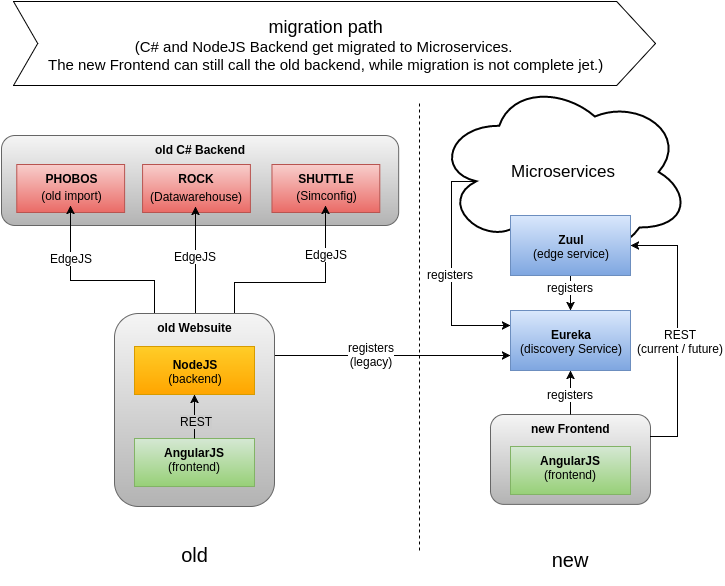
\includegraphics[width=1\textwidth]{res/Websuite_migration}
	\caption{Websuite migration path}
	\label{fig:websuite-migration}
\end{figure}

The old JavaScript stack, containing of an AngularJS front-end and an NodeJS back-end with connections to the C$\sharp$ code, over EdgeJS was replaced. The NodeJS components were migrated to several micro-services and the front-end was converted to a WebUI micro-service that consists of an AngularJS front-end with a thin layer of NodeJS to host the application.\\
The process of migrating to the new structure is complete and the old monolithic Websuite is not used anymore.



\section{Tooling}
To effectively develop a front-end application, certain tasks have to be done, to make the process convenient in development and usable in production. The following topics have to be considered.


\subsection{Dependency management}
Almost every application depends on third-party components. Manually managing dependencies is an error prone tasks and checking them into the version control system clutters its history.\\
This is why the WebUI uses the \textit{Node Package Manager} (NPM) and Bower. NPM is responsible for managing NodeJS dependencies that are used for tooling and serving the Angular app. Bower takes care of the front-end libraries. Both tools depend on a JSON file that lists the needed dependencies, as well as their required version. This guarantees that any deployment of the app uses the correct version of any used library.


\subsection{Task Runner}
A task runner allows to run various tasks that are used during the development process. The WebUI uses Gulp, which is responsible for executing the following tasks.

\subsubsection{Live reload} Restarts the application and reloads the website inside the browser, once the source code has changed. It is only used for development.

\subsubsection{Browser sync} Synchronizes the active state of all open browser windows. This helps testing cross-browser compatibility in development.

\subsubsection{Combining files} Combines all files of a type (e.g. .js, .html or .css) to one file. This reduces the amount of connections needed to serve the page in production and therefore improves load time.

\subsubsection{Uglifying} Renames variables and functions to single character names to reduce the size of the served files in production.

\subsubsection{minifying} Removes spaces and line-breaks, to further reduce the file size in production.

\subsubsection{Compiling SCSS}
Compiles the SCSS styles to CSS. For further information see section \ref{sec:styling}.


\subsection{Initial Configuration}
\label{sec:initial_config}
The tasks above need to be configured, to match the development work-flow and the used file structure. This initial configuration was created with a tool called \textit{generator-gulp-angular} and modified to match the actual need for the WebUI. Additionally the generator created the file structure, used by the new WebUI.



\section{Migrating the application}
While it was possible to strip out old parts and reuse the old Websuite's code-base, this was not done. Instead, a completely new structure with tested tooling was created, using the previously mentioned generator-gulp-angular (see section \ref{sec:initial_config}). This guaranteed that no old code was left inside the application, which could cause problems in the future.\\


\subsection{Components}
In the migration process, the following components were migrated.

\subsubsection{Import}
\begin{figure}[H]
	\centering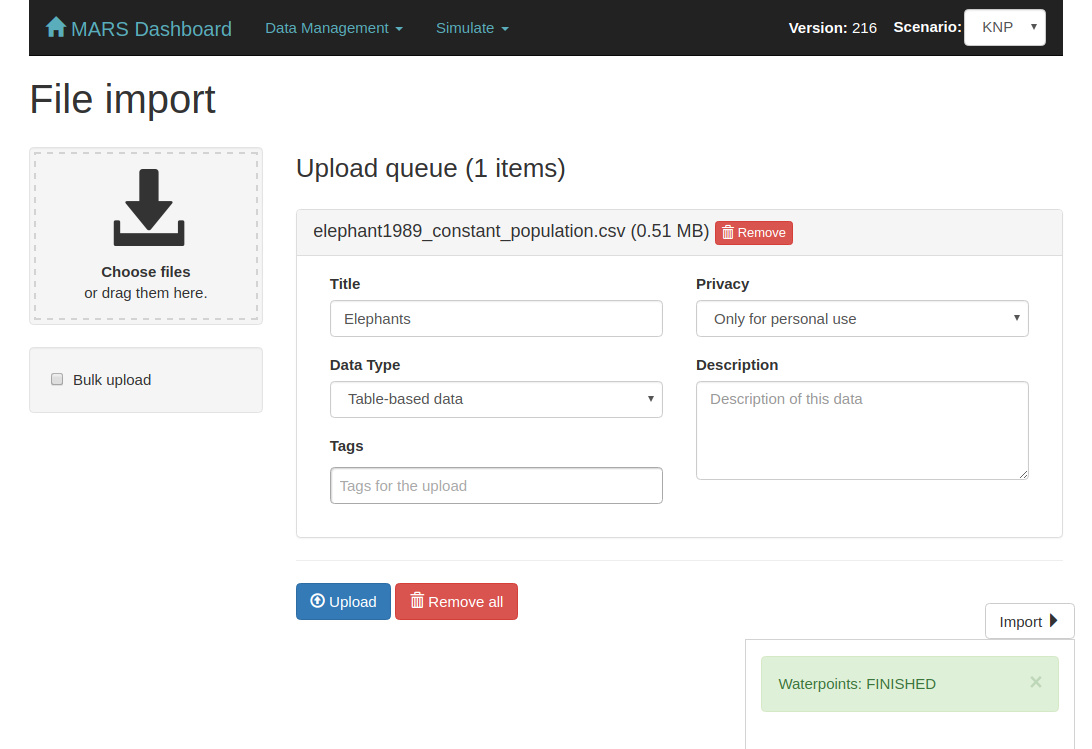
\includegraphics[width=1\textwidth]{res/import-ui}
	\caption{Import UI}
	\label{fig:import-ui}
\end{figure}
As part of the the migration, the two imports \textit{data} and \textit{model} were migrated to one code-base. This was done, by creating an import directive that can be parameterized upon usage. The merge eliminated duplicate code and resolved already existing variation in the behavior of the imports.\\
The process that is shown in figure \ref{fig:import} shows the way, the import interacts with the back-end. Once the user selects one or more files, the WebUI generates one input form for every file. An exception is the \textit{bulk upload}. If this option is enabled, one form is generated for all files. The forms are validated while the user inputs data, to prevent mistakes as early as possible.\\
Once the user starts the upload, the files are successively send to the \textit{file service}. During that process the upload progress is shown. When the file have been uploaded, the WebUI triggers the long-polling (see section \ref{sec:long-polling} for more detail). This is done independent of the the import page and the current state is therefore visible from any page. This also means that the user may leave the page and come back later to check, if the processing was successful. The UI of this import is shown in \ref{fig:import-ui}.

\begin{figure}[H]
	\centering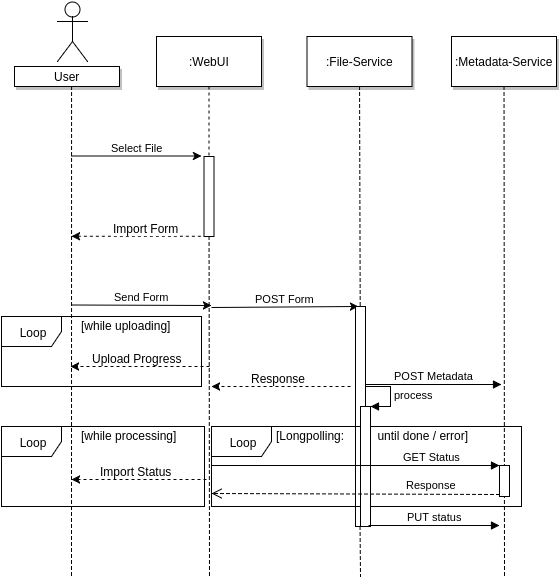
\includegraphics[width=.75\textwidth]{res/Import}
	\caption{Import sequence diagram}
	\label{fig:import}
\end{figure}


\subsubsection{Data View}
The migration of the data view did not require any special changes. The REST calls were extracted, the CSS was cleaned up and the code was refactored to improve the maintenance.

\subsubsection{Scenario Creation}
The Scenario Creation is a new component that did not exist in this form previously. Its only purpose is to list existing scenarios and allow the creation of new once. When creating a new scenario, a model is specified. The Scenario-management-service adds the mapping fields, based on the models reflection result. This is used in the mapping component. Once a new scenario has been created, the list of scenarios gets refreshed. The whole work-flow is shown by figure \ref{fig:scenario}.
\begin{figure}[H]
	\centering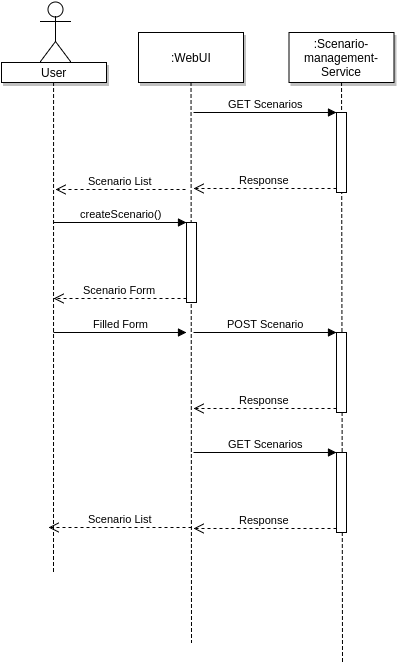
\includegraphics[width=.60\textwidth]{res/Scenario}
	\caption{Scenario}
	\label{fig:scenario}
\end{figure}

\subsubsection{Mapping Creation}
The mapping creation replaces the old, domain-specific language based mapping component. When a scenario is selected, the required mapping fields and parameters are requested from the scenario-management-service.\\
From this structure, the mapping page is generated. Based on the currently selected field of a layer, the mappable data is filtered, to only allow mapping of matching types.\\
When the user triggers a mapping action, the fields containing reference to the data are added to the mapping structure. This depends on the type of data, e.g. for table data, the following fields have to be added: \textit{tableName}, \textit{columnName}, \textit{columnClearName} and \textit{dataId}. Once a field is mapped, the next is automatically selected.\\
Once a save is triggered, the data is sent to the scenario-management-service and the mapping is refreshed. This refreshed mapping structure contains the validation result for the mapped fields. Additionally, the current progress of mapping is displayed. This shows the number of fields that failed the validation. A list is available that shows the reason a specific mapping failed. Figure \ref{fig:mapping} shows the calls needed for the just described process.
\begin{figure}[H]
	\centering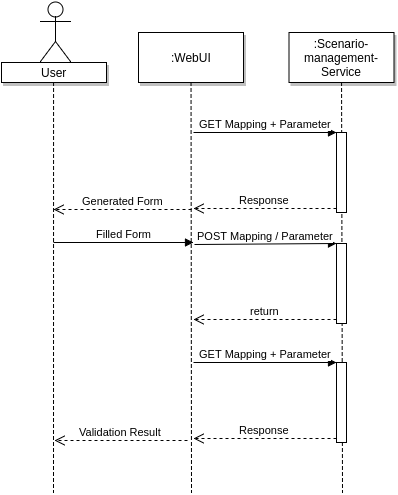
\includegraphics[width=.65\textwidth]{res/Mapping}
	\caption{Mapping}
	\label{fig:mapping}
\end{figure}


\subsection{Long-polling}
\label{sec:long-polling}
Long-polling is used between the WebUI and the Metadata Service to report the current processing status of an import.\\
To trigger long-polling, the WebUI sends an GET request to the \textit{Metadata Service} and and \enquote{init} as the current state. The server responds with the current state and the WebUI from now on sends a new request, every time it receives a response, appending the current state. The Metadata Service delays the answers, until the state has changed. This process is repeated until the import is either successful or failed.\\
The goal was to always have the current state, without having to constantly poll the back-end. The way HTTP calls work, does not allow the server to send a message to the client, without a previous request. This can be solved by sockets. For technical reasons, this was not an option. Therefore long-polling is the best solution for the moment.

\subsection{Boundary Factories}
During the migration, all REST calls were extracted into factories. They serve as a boundary to other services and are the single point that communicates to other components. This means, they execute REST calls to the back-end services and interact with the browsers local storage to persist certain settings (e.g. the selected scenario).\\
Besides executing the actual REST calls, the factories are responsible for converting remote inputs to the local structure and vice versa.\\
This design ensures that API changes need to be adopted at one single place which holds the truth for all data coming in and out of the WebUI.


\subsection{Error Handling}
The WebUI is the component that stands between the user and the back-end services. Therefore it is essential, to provide the user with proper feedback, if an error accrues.\\
This is why, an error factory exists that gives an easy way to generate user feedback. The input is a mandatory error message and an optional error type. The type controlles the color of the feedback. Once invoked, an error message is displayed with a button to discard it. The messages are also distinct, which prevents duplicate messages. The following listing shows an example. 
\begin{lstlisting}[language=javascript, caption=error handling]
vm.alerts.add('it worked', 'success');
vm.alerts.add('it worked', 'success');
vm.alerts.add('this looks weird', 'warning');
vm.alerts.add('implicit default');
vm.alerts.add('Something went wrong', 'danger');
\end{lstlisting}

% TODO: result image


\subsection{Styling}
\label{sec:styling}
The styling of the old application was discarded, because it contained many lines of self-written CSS that had no unified look and was not responsive for the most part. Instead the layout is done using bootstrap with minimal adjustments at certain points.\\
To prevent visual side effects in other components, every html template is wrapped in a div, with its components name as the id. The CSS file for every component is only applied to children of this id.\\
To further improve the simplicity of the styling \textit{Sassy CSS} (SCSS) was used to write styles. SCSS is a CSS preprocessor that is compiled to CSS and adds features like variables, reusable components, loops and nesting.\\
The fact that it uses CSS syntax, allows a smooth transition, because the developer can use it like normal CSS and make use of the additional features when ever he desires.
